\documentclass[a4paper,11pt]{article}
\usepackage[utf8]{inputenc}
\usepackage{lastpage}
\usepackage{fancyhdr}
\usepackage[english]{babel}
\usepackage[a4paper,margin=1in]{geometry}
\usepackage[table,xcdraw]{xcolor}
\usepackage{array}
\usepackage{amsmath}
\usepackage{amssymb}
\usepackage{graphicx}
\usepackage[numbered,framed]{matlab-prettifier}
\usepackage{minted}


\newcommand\tab[1][4mm]{\hspace*{#1}}
\newcommand{\norm}[1]{\left\lVert \mathbf{#1} \right\rVert}
\newcommand{\abs}[1]{\left\vert #1 \right\vert}

%-------------------------------------------------------------------------------
% HEADER & FOOTER
%-------------------------------------------------------------------------------

\pagestyle{fancy}
\fancyhf{}
\setlength\headheight{15pt}
\fancyhead[L]{MCSC 6230G Assignment 1 }
\fancyhead[R]{Student ID: 100633486}
\fancyfoot[R]{Page \thepage\ of \pageref{LastPage}}


%-------------------------------------------------------------------------------
% TITLE PAGE
%-------------------------------------------------------------------------------

\begin{document}

\title{
	\Huge \textbf {Advanced Topics in High-Performance Computing}
    \\ [0.2cm]
	\LARGE Assignment 1, October 2017
    \\ [0.5cm]
    \hrule
}

\date{}

\author{
		\Large Kamyar Nazeri \\
		\large Student ID: 100633486 }

\maketitle


\newpage

\section{Introduction.}
In this assignment we train a linear regression model to predict house prices using housing data. We will be using California housing dataset from StatLib. The dataset consists of 20,640 average house values as target variables and 8 features: \textit{average income, housing average, age, average rooms, average bedrooms, population, average occupation, latitude}, and \textit{longitude}. \\
We employ Ridge Regression (\textit{Tikhonov} regularization) to find the best estimate of the true value of the housing price. We start with a linear model and try to find the best regularization hyper-parameter using cross-validation and plot the corresponding train and test errors. We will compare these results with models using higher degree polynomial of features and finally suggest the best model for predicting housing price for our dataset.

\section{Procedure.}
We will be using Normal Equation to minimize the least square error and find the best estimate of the true value of the housing price: \\
\begin{align*}
\operatorname*{argmin}_\theta\bigg(\norm{y-X\theta}_2^{2} + \delta^2\norm{\theta}_{2}^2\bigg)
\end{align*}
\noindent
With $\mathbf{X}$ being the design matrix with each row as a data point and each column representing a feature. 
The first step is to whiten our data; Data whitening is a decorrelation transformation that transforms our features into a set of new features with identity covariance (uncorrelated with unit variances): 
\begin{align*}
\mathbf{X}_{whitened}^T = (\mathbf{X}^T\mathbf{X})^{-\frac{1}{2}}\mathbf{X}^T
\end{align*}
\\The python code to whiten the data is as follows:

\begin{minted}{python}
   X_whiten = sc.linalg.inv(sc.linalg.sqrtm(X.T.dot(X))).dot(X.T).T
\end{minted}

\noindent
\\Next, we add the intercept column to our design matrix to represent the bias:
\begin{align*}
\mathbf{X}_{intercept} = [\mathbf{1}\ \vert\ \mathbf{x_1}\ \vert\ \mathbf{x_2}\ \vert\ ...\ \vert\ \mathbf{x_n}]\ \in \ \mathbb{R}^{m\times (n+1)}
\end{align*}
With $m$ being the number of training examples and $\mathbf{x_1}\ ...\ \mathbf{x_n}$ column vectors representing each feature in our dataset. 
\\The python code to add the intercept column is as follows:

\begin{minted}{python}
   X_intercept = np.c_[[1] * X_whitened.shape[0], X_whitened]
\end{minted}

\noindent
\\We apply normal equation on the design matrix to find the parameters estimating our data:
\begin{align*}
\theta = (\mathbf{X}^T\mathbf{X}+\delta^2\mathbf{I}_{(n+1)})^{-1}\mathbf{X}^T\mathbf{y}
\end{align*}
With $\delta^2$ being the regularization term and $\mathbf{I}_{(n+1)}$ an identity matrix. We need to make sure that we do not regularize the bias term, meaning in the equation above we replace $\mathbf{I}_{(n+1)}$ with $\mathbf{\tilde{I}}_{(n+1)}$ with the following structure:
\begin{align*}
\mathbf{\tilde{I}}_{(n+1)} = \mathrm{diag}\big\{0, 1, 1, ..., 1\big\}\ \in\ \mathbb{R}^{(n+1)\times(n+1)}
\end{align*}
In other words, the first entry of the matrix $\mathbf{\tilde{I}}_{(n+1)}$ is \textbf{zero}:
\begin{align*}
\theta = \Biggl(\mathbf{X}^T\mathbf{X} + \delta^2 \begin{bmatrix}
0 & & & \\
& 1 & & \\
& & \ddots & \\
& & & 1
\end{bmatrix}\Biggl)^{-1}\mathbf{X}^T\mathbf{y}
\end{align*}

\noindent
\\The python function to solve the Ridge Regression for $\theta$ is as follows:

\begin{minted}{python}
import numpy as np
import scipy as sc

def estimate_theta(X, y, d2):
	m, n = X.shape
	reg = d2 * np.eye(n + 1)    # regularization
	reg[0, 0] = 0	       # not regularizing the bias           
	
	# solve the normal equation
	theta = np.linalg.inv(X.T.dot(X) + reg).dot(X.T.dot(y))
	return theta
\end{minted}

\section{Ridge Regression Results}
\subsection{\large Regularization Paths:}
Our first task is to plot values of $\theta$ for different values of $\delta^2$. The range of regularization term is from $10^{-7}$ to $10^{-1}$:
\begin{figure}[!htb]
	\centering
	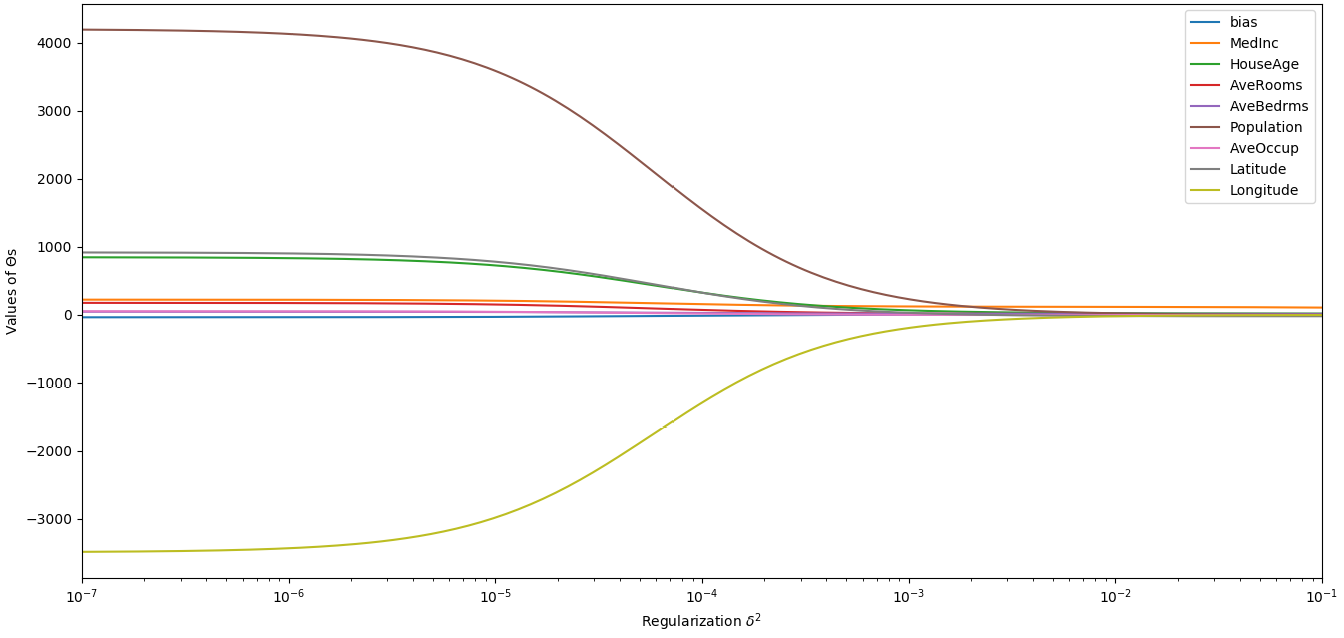
\includegraphics[width=17cm, height=8.5cm]{plotA.png}
	\caption{\small Ridge coefficients as a function of the regularization.}
\end{figure}
\\The plot shows that as the regularization term increases, the coefficients are heavily penalized hence become smaller; As a result, the hypothesis will be approximately equal to the bias term.

\subsection{\large Error Analysis:}
\noindent
To calculate error of the Ridge Regression model, we ue Mean-Square-Error, with $y^{(i)}$ being the $i^{th}$ label and $\mathbf{x}^{(i)}$ being the $i^{th}$ data-point:
\begin{align*}
MSE = \frac{1}{m}\sum\limits_{i=1}^{m}(y^{(i)}-\theta^T\mathbf{x}^{(i)})^2
\end{align*}
\noindent
\\We split the data into training (80\%) and test(20\%) sets (80/20 is indeed a good starting point) and calculate MSE for a range of regularization hyper-parameter from $10^{-7}$ to $10^{3}$:
\begin{figure}[!htb]
	\centering
	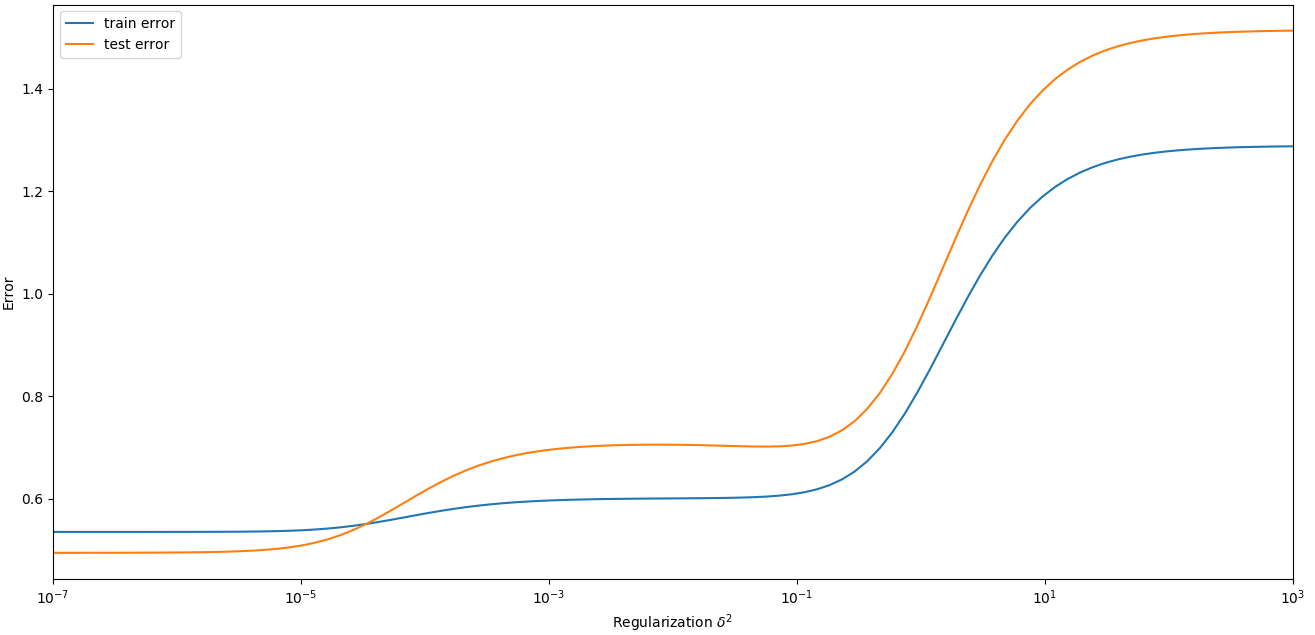
\includegraphics[width=15cm, height=7cm]{plotB_without_shuffle.png}
	\caption{\small Comparison of test and train error for different values of regularization.}
\end{figure}
\\\\To avoid any element of bias/patterns in the split datasets we shuffle data before training; This can break any possible correlation among the features and the MSE error becomes:
\begin{figure}[!htb]
	\centering
	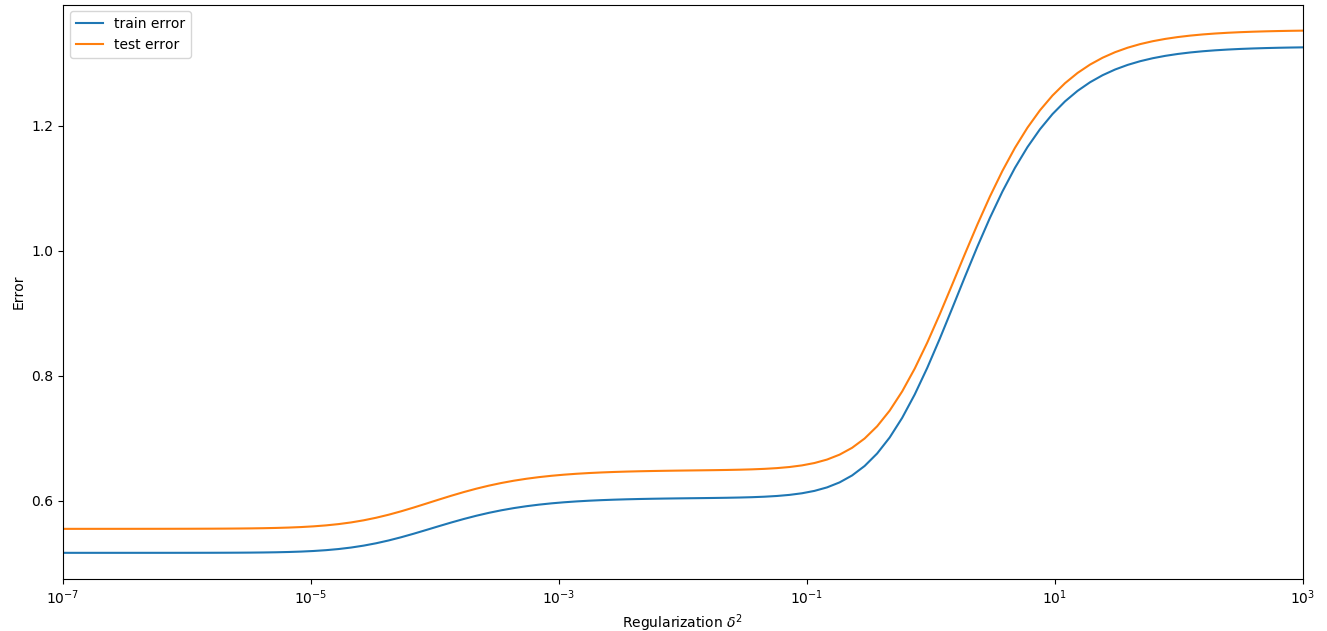
\includegraphics[width=15cm, height=7cm]{plotB.png}
	\caption{\small Comparison of test and train error for different values of regularization with shuffling}
\end{figure}
\noindent
\\We use \textit{scikit} built-in functions to shuffle data:
\begin{minted}{python}
   X, y = sklearn.utils.shuffle(X, y)
\end{minted}
To decrease the correlation in data even more and come up with the best cross validation we tried 5-fold cross validation on the shuffled data and took the average from the folds. The test error becomes smoother in the following plot:
\begin{figure}[!htb]
	\centering
	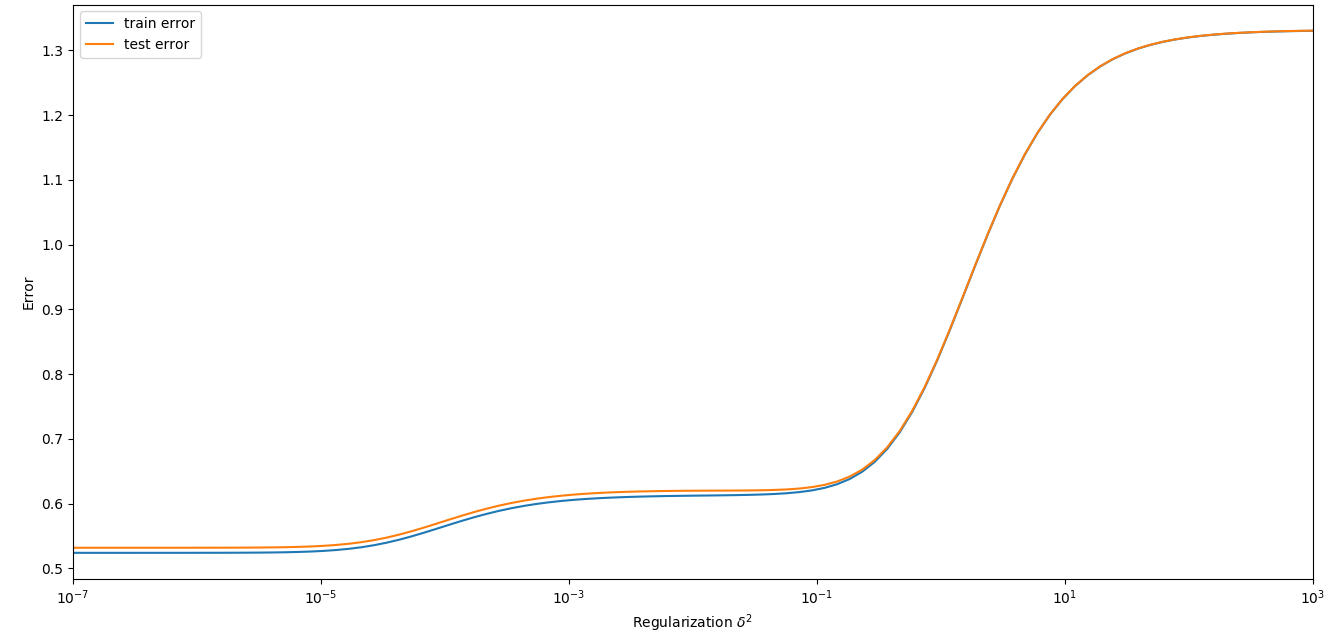
\includegraphics[width=15cm, height=7cm]{plotB_5fold.png}
	\caption{\small Comparison of test and train error for different values of regularization with shuffling and 5-fold cross validation}
\end{figure}
\noindent
\\The errors graph in \textit{figures 2-4} show that as we increase the value of regularization $\delta^2$, the model becomes high bias and eventually underfits the data, this model is very simple that the hypothesis is almost equal to the bias term. \\
The best regularization hyper-parameter in our model is any value less than $10^{-5}$ where the test and train errors are at their minimum. Any regularization value greater than that would have a negative effect on the error. This model would work just fine even without regularization ($\delta^2=0$) however, to generalize our model to polynomial regression we chose to include the regularization value. \\

\subsection{\large Best Model:}
To select the best model for our regression problem, we also tried degree 2 and 3 polynomial of features; choosing higher degree polynomials (n $>$ 3) would result in numerical instability when finding the inverse of a matrix in the normal equation with a whitened data. \\
The following are the same regression model on the \textit{Population} feature in our dataset using first order, degree 2 and 3 polynomials: 
\begin{figure}[!htb]
	\centering
	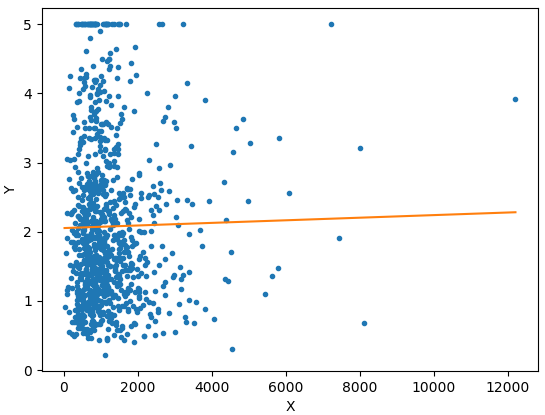
\includegraphics[width=.3\textwidth]{linear_d1.png}\hfill
	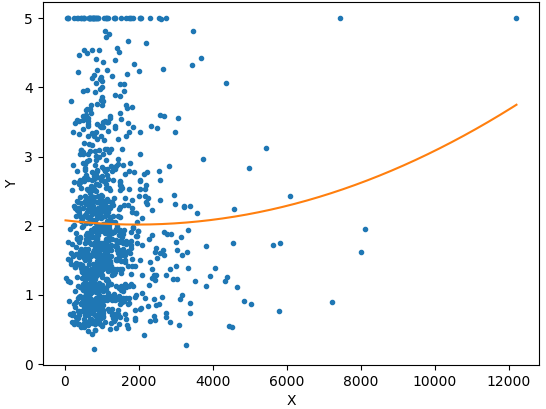
\includegraphics[width=.3\textwidth]{linear_d2.png}\hfill
	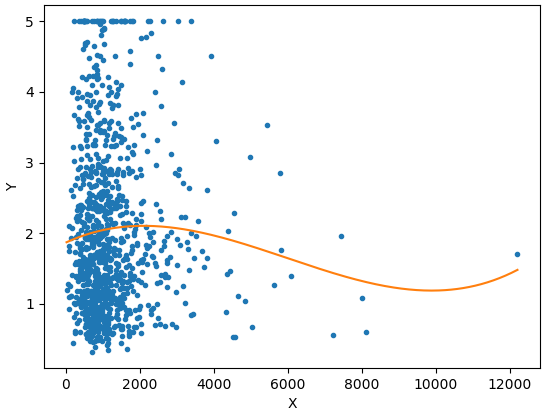
\includegraphics[width=.3\textwidth]{linear_d3.png}
	\caption{Price of the house as a function of Population. left: 1st order, middle: 2nd degree, right: 3rd degree}
\end{figure}
\\\\The 3rd degree polynomial feature might be able to fit the data much better by smoothing the regression curve; however, we need to regularize it well enough to prevent overfitting. The following plot shows the 3rd degree polynomial test/train MSE for different values of regularization:

\begin{figure}[!htb]
	\centering
	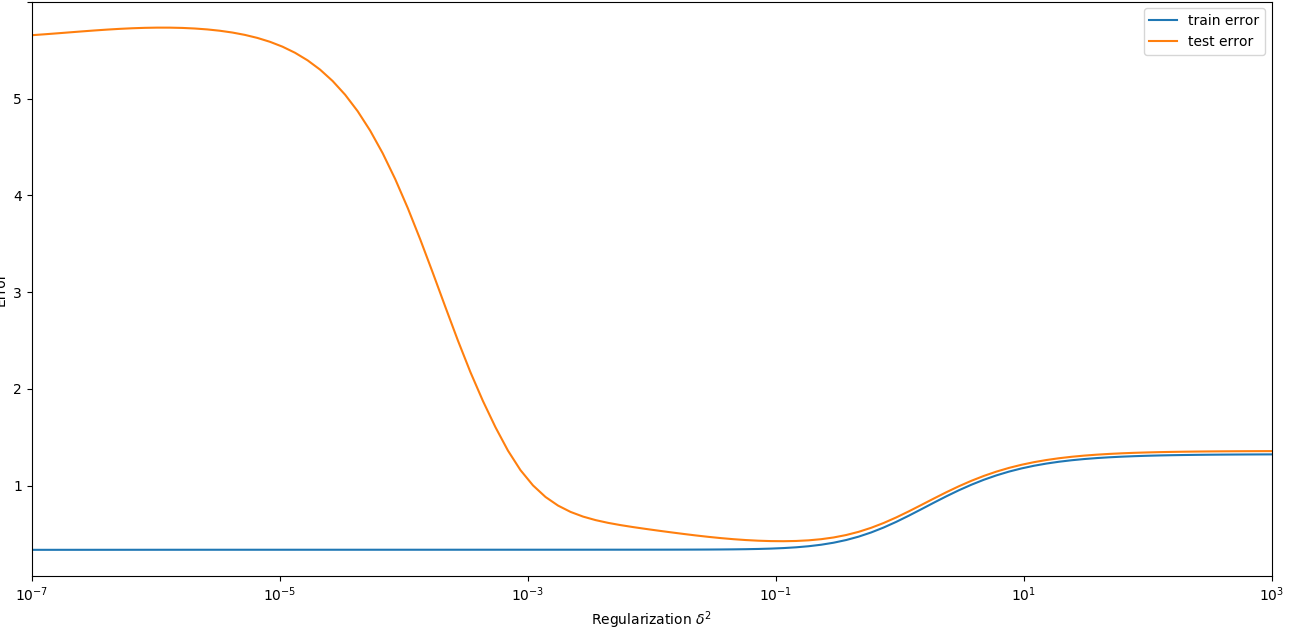
\includegraphics[width=15cm, height=7cm]{plotB_3_1.png}
	\caption{\small Comparison of test and train error for different values of regularization with 3rd degree polynomial features}
\end{figure}
\noindent
\\ The errors graph in \textit{figure 6} suggests that although with higher degree polynomial the error is relatively smaller compared with the first order features, the system is more prone to overfitting. Regularization becomes necessary with polynomial regression, otherwise the test error becomes large and the model becomes high variance. The best regularization value in the model above (3rd degree) is almost $10^{-1}$. \\
This simple experiment shows that as long as we regularize, higher degree models could outperform linear models in terms of mean-square error.



\section{Conclusion.}
Linear regression attempts to draw a straight line that best minimizes the residual sum of squares between the data points and the predictions. However, this model does not generalize well and is prone to overfitting, especially with higher degree polynomial of features(\textit{figure 6}, $\ \delta^2<10^{-1}$). With Ridge Regression we penalize a least squares by shrinking the values of the coefficients; Using regularization, the slope of the regression line tend to be more stable and the variance smaller (\textit{figure 6}, $\ \delta^2=10^{-1}$). \\\\
Considering the values of $\theta$ (\textit{figure 1}) one can conclude that the most important feature in our regression model is \textit{Population}. This is based on the idea that when a range of independent features are all on the same scale, the most important features should have the highest coefficients ($\theta$) in the model. In our model, features with the most impact on the housing price are: \textit{Population, Latitude, HouseAge, MedInc, AveRooms, AveOccup, AveBedrms}, and \textit{Longitude} respectively.

\end{document}
